\documentclass[12pt, a4paper,titlepage,openright,twoside]{report}
\usepackage[english]{babel}%divisione in sillabe
\usepackage[utf8]{inputenc}%caratteri accentati
\frenchspacing%spaziatura latina
%\usepackage[Glenn]{fncychap}
%\usepackage[T1]{fontenc}
%\usepackage[Lenny]{fncychap}
%\ChNameVar{\fontsize{14}{16}\usefont{T1}{cmr}{m}{n}\selectfont}
%\ChNumVar{\fontsize{60}{62}\usefont{T1}{cmr}{m}{n}\selectfont\color{black}}
%\ChTitleVar{\Huge\bfseries\rm}
% \ChRuleWidth{1pt}
\usepackage{fancyhdr}
\usepackage{color}%altri di LyX
\usepackage{amstext}
\usepackage{amssymb}
\usepackage{graphicx}%altri di cri
\usepackage{amsmath,enumerate,rotate}
\usepackage{epsfig}
\usepackage[width=125mm]{caption}
\usepackage{subfig}
\usepackage{indentfirst}
\usepackage{booktabs}
\usepackage{graphicx}
\usepackage{tabularx}
\usepackage{float}
\usepackage{xcolor,calc, blindtext}
\usepackage{cite}
%\usepackage{url}
%\Urlmuskip=0mu plus 1mu
%\usepackage{kpfonts}
%\setSingleSpace{1.1}
%\SingleSpacing
\usepackage[breaklinks=true]{hyperref}
\usepackage{breakurl}
\usepackage{listings}
\usepackage[nottoc,notlot,notlof]{tocbibind}
%##############################################################################################################################
\newcommand{\comment}[1]{}
\renewcommand{\kappa}{\mathsf k}
\newcommand{\Esse}{\mathcal S}
\newcommand{\Elle}{\mathtt L}
\newcommand{\Ee}{\mathtt E}
\newcommand{\enne}{\mathfrak n}
\newcommand{\di}{\mathtt d}
\newcommand{\Enne}{\mathcal N}
\newcommand{\emme}{\mathfrak m}
\newcommand{\elle}{\mathnormal l}
%##############################################################################################################################
\lstdefinestyle{customc}{
	belowcaptionskip=1\baselineskip,
	breaklines=true,
	frame=L,
	tabsize=2,
	numbers=left,
	xleftmargin=\parindent,
	language=C++,
	showstringspaces=false,
	basicstyle=\footnotesize\ttfamily\scriptsize,
	keywordstyle=\bf,
	commentstyle=\textit,
%	identifierstyle=\color{blue},
%	stringstyle=\color{orange},
}

\comment{
\definecolor{chaptercolor}{gray}{0.8}
% helper macros
\newcommand\numlifter[1]{\raisebox{-2cm}[0pt][0pt]{\smash{#1}}}
\newcommand\numindent{\kern37pt}
\newlength\chaptertitleboxheight
\makechapterstyle{hansen}{
  \renewcommand\printchaptername{\raggedleft}
  \renewcommand\printchapternum{%
    \begingroup%
    \leavevmode%
   \chapnumfont%
    \strut%
    \numlifter{\thechapter}%
    \numindent%
\endgroup%
}
  \renewcommand*{\printchapternonum}{%
    \vphantom{\begingroup%
      \leavevmode%
      \chapnumfont%
      \numlifter{\vphantom{9}}%
      \numindent%
      \endgroup}
    \afterchapternum}
  \setlength\midchapskip{0pt}
  \setlength\beforechapskip{0.5\baselineskip}
  \setlength{\afterchapskip}{3\baselineskip}
  \renewcommand\chapnumfont{%
    \fontsize{4cm}{3cm}%
    \bfseries%
    \sffamily%
    \color{chaptercolor}%
  }
  \renewcommand\chaptitlefont{%
    \normalfont%
    \huge%
    \bfseries%
    \raggedleft%
  }%
  \settototalheight\chaptertitleboxheight{%
    \parbox{\textwidth}{\chaptitlefont \strut bg\\bg\strut}}
  \renewcommand\printchaptertitle[1]{%
    \parbox[t][\chaptertitleboxheight][t]{\textwidth}{%
      %\microtypesetup{protrusion=false}% add this if you use microtype
      \chaptitlefont\strut ##1\strut}%
}}
\chapterstyle{hansen}
%\aliaspagestyle{chapter}{empty} % just to save some space
}
%############################################################################
\pagestyle{fancy}
\renewcommand{\chaptermark}[1]{\markboth{#1}{}}
\renewcommand{\sectionmark}[1]{\markright{\thesection\ #1}}
\fancyhf{}
\fancyhead[LE,RO]{\itshape\thepage}
\fancyhead[RE]{\itshape\footnotesize\nouppercase{\leftmark}}
\fancyhead[LO]{\itshape\footnotesize\nouppercase{\rightmark}}
%##############################################################################################################################
\begin{document}
	\pagenumbering{roman}
\title{\huge \textbf{Models for hierarchical inheritance structures in object-oriented programming languages}}
\author{Mariacristina Romano\\
Dipartimento di Fisica, Universit\`a degli Studi di Milano,\\
Via Celoria 16, 20133 Milano, Italia}
%---------------------------------------------------------
{
\thispagestyle{empty}

\centerline{
\includegraphics[width=120mm,angle=0,clip=]{images/UniversitasMediolanensis.eps}
}

\begin{center}
{\large Facolt\`a di Scienze e Tecnologie\\
\vskip0.2cm Laurea Magistrale in Fisica }
\end{center}


\vskip1.5cm
\begin{center}
\huge \textbf{Models for hierarchical inheritance structures in object-oriented programming languages}
\end{center}

{\large
\vskip20mm Advisor:  Prof. Mario Raciti
\vskip 1mm Co-advisor: Prof. Marco Gherardi\\
}

\vskip0.7cm
\hskip8cm\parbox[t]{7cm}
{\large 
Mariacristina Romano\\
Matr. n$^\circ$ $823029$\\
A.Y. $2013$/$2014$\\
\vskip 0.5mm PACS: 89.75.-k
}

\newpage
\newpage
\thispagestyle{empty}
\clearpage
}

 % qui include il frontespizio
\date{April 15, 2015}
\newpage\null\thispagestyle{empty}\newpage %pagina bianca dopo il mio frontespizio
\thispagestyle{empty}
%---------------------------------------------------------
%\begin{flushright}
%\null\vspace{\stretch{1}}
%{\textit{A me}}
%\vspace{\stretch{2}}\null
%\end{flushright}
%---------------------------------------------------------
%\newpage\null\thispagestyle{empty}\newpage
\maketitle
\newpage\null\thispagestyle{empty}\newpage
%---------------------------------------------------------
\begin{abstract}
\center
Object-oriented programming languages allow developers to write software in which \textit{objects} have different kinds of relations and interactions: a complex system!

\vspace{0.5cm}
The object paradigm states a list of rules which facilitate the code re-use. Probably the most important mechanism that leads to a minimal effort is the inheritance relation.

\vspace{0.5cm}
Inheritance allows the construction of multilevel hierarchies, which can be modeled by directed acyclic graphs.

\vspace{0.5cm}
How do programmers use inheritance? Which kind of graphs arise from hierarchical relations? What quantity governs the optimization?

\vskip1.75cm
\hskip4.5cm
\parbox[b]{7cm}
{
Advisor: {\textit Prof. Mario Raciti}\\
Co-advisor: {\textit Prof. Marco Gherardi}
}
\end{abstract}
%--------------------------------------------------------
\newpage\null\thispagestyle{empty}\newpage
\tableofcontents
\newpage\null\thispagestyle{empty}\newpage
%##############################################################################################################################
%##############################################################################################################################
%##############################################################################################################################
\clearpage{\pagestyle{empty}\cleardoublepage}
\chapter{Object-oriented paradigm}
	\pagenumbering{arabic}
%******************************************************************************************************************************
Object-oriented programming is the most used programming paradigm in today software design. It allows an intelligent code reuse through inheritance and polymorphism, and it is probably the only one programming paradigm that allows people to design huge projects with a cooperative effort.

Programs and libraries written in object-oriented languages are composed through the concept of \textit{objects}, which can be seen as modular code, composed by data and methods. Objects can interact with each other and there may be different kinds of relations among them.

Through the concept of objects, the whole set of programs can be seen as a huge complex system, with many small elements which interact and cooperate to achieve the same goal, which is the purpose for which each program has been made.

One of the most important relation that can bind objects is the inheritance: a rule introduced in object-oriented programming languages in order to facilitate and automate the reuse of code.

The relation of inheritance arranges objects in hierarchies: when an object inherits from another one, we can imagine a small graph with two nodes connected by a directed link, for example from the original object to the one which has inherited the code. Then, we can add lots of other objects to such graph, and make it enormous and complex, due to the possibility to inherit code from different objects and due to the fact that there is no limitation in the number of objects that can inherit code from the same object.

Such hierarchies are the starting point of this work.

\section{A little terminology}
\subsubsection{Class and objects}
Object is the word used to refer to an instance of a \textit{class}: there may be lots of objects of the same type in a program. In this thesis there is no necessity to distinguish these two concepts and words will be used without distinctions.

\subsubsection{Abstract classes}
An abstract class is a class that can not be instantiated and so that can never become an object. Such class contains methods that has no implementation, but only a declaration.

\subsubsection{Superclasses and subclasses}
When a class inherits from another class, the first is called the \textit{superclass} of the second one, while the second is a \textit{subclass} of the first one.

The subclass usually inherits from the superclass its \textit{public code}.

\subsubsection{Multiple Inheritance}
Multiple inheritance occurs when a subclass has more than one superclass. Many programming languages allow this possibility, like C++ and Python, while in others it is limited (as in Java) or even not allowed.

\subsubsection{Multilevel Inheritance}
Multilevel inheritance occurs when a subclass has inherited from one (or more) superclass which is itself the subclass of another class.

In all programming languages studied in this thesis, multilevel inheritance is enabled, but there is a way to prevent the inheritance from a class in Java and C++, through a specific keyword inserted in the class that is considered \textit{final} for the hierarchy.
\newpage
\section{Object-oriented programming languages}
There are many object-oriented programming languages, with lots of differences among them but united by the object paradigm. To give a complete overview of inheritance hierarchies, three different programming languages have been analized: C++ \cite{cpp}, Java \cite{java} and Python \cite{python}.

This thesis can not contain a whole course about three programming languages, but it is useful, however, to highlight some important differences, in order to give you the tools to judge the data analysis.

\subsubsection{C++ language}
Among the three languages, C++ is the oldest and the one which spread the object-oriented paradigm.

It has been designed to improve \textit{C language}, adding features as virtual functions, operator overloading, references, keywords to control the store-free of memory, and, obviously, the object-oriented paradigm.

It is a typed language and it supports multiple inheritance.

\subsubsection{Java language}
Java has been designed to be a secure and portable programming language.

Its syntax is identical to the one of C++, but its inheritance rules has some peculiarity. Multiple inheritance is not available in the common sense: a class can inherit code from one superclass only, but it can also inherit declarations of functions and variables from any number of a special kind of classes, called \textit{interfaces}.

In general, rules have been created in order to reduce complexity in programs and to keep the code as simple as possible without limiting its capabilities. Some examples are the prohibition to overload operators, the deletion of the instruction \textit{go to} and of the multiple inheritance.

\subsubsection{Python language}
Python has been designed with the goals of be useful in any purpose and to allow a really fast programming.

The syntax is quite different respect to the other two languages, since its design philosophy is to allow to express concepts in the minimum possible lines of code and since it is strongly dynamically typed.

It allows multiple inheritance as well as C++, without any limitation.

\section{Complex noisy data}
A complex system analysis always begins from a set of chaotic, complex and noisy data.

Internet is the open-source code home and allows people to obtain a huge amount of libraries and programs in every programming language. The noisy data, which is the subject of the following analysis, has been downloaded from GitHub \cite{gith}, the largest code hoster in the world \cite{gitworld}.

Hierarchical inheritance structures can be easily modeled as directed acyclic graphs, and then the dataset is a huge ensemble of different kinds of graphs.

In graphs terminology, the oudegree of a node is the quantity which describes the number of nodes pointed by a link from such node. Since it describes how many classes inherit from such class, such relation means speciation.

The indegree instead represents the multiple inheritance, and so it describes the number of classes from which the selected class has inherited code.

Another important point is that each program is made to perform a task, and then each hierarchy is done to solve a problem or a subtask of the whole program.

In principle all classes in a hierarchy can be directly used in programs, excluding abstract classes, but only some of these classes becomes real objects, while the other nodes have structural purposes only.

%
%
%
%
%


%******************************************************************************************************************************
\newpage
\clearpage{\pagestyle{empty}\cleardoublepage}
\newpage
\chapter{Minimal Effort model}
	\label{Ceffort}
%******************************************************************************************************************************
The dataset is large and noisy. A model is needful to guide the data analysis and to give an interpretation to all results.

The guiding idea of the Minimal Effort model is that inheritance is designed to better promote code reuse and, in this sense, to minimize the effort in writing programs.

The model is a mean field approximation for graphs and it allows you to obtain some interesting features, useful in all next chapters. 

%******************************************************************************************************************************
\section{Reuse and Effort}
Programs are created to perform tasks and solve problems and, in object-oriented programming, each task is performed with modular code, the objects, often organized in hierarchies.

In a first approach, let's suppose that only terminal nodes of inheritance graphs compose the effective solution of the problem, while all nodes at higher levels are made for code reuse purposes only.

Terminal nodes are the leaves of the tree which represents the hierarchy. Leaves are given by the problem, but rules are needed in order to build the whole tree from its leaves. How can we group leaves in different levels? Which principle may guide us?

\subsection{Why use inheritance?}
Assuming that inheritance most important effect in graph structure is code reuse, we can start from the $\enne$ classes which represent the solution of the problem.

Suppose that the implementation of two of this classes is very similar. Then you can move mutual code lines in a third node, in the upper level of this tree.

In this way, one can avoid writing twice the mutual lines, creating a node which shares its lines with the two leaves. In this sense, we are guided by a minimum effort principle. Obviously, one can group more than two nodes and try to absorball mutual lines of leaves code in higher level.

The function effort $\Ee$ of a tree is defined simple as
\[ \Ee = \sum_{\sigma}^{\enne} \text{cost}(\sigma) \]
a sum over all nodes, were each node cost is normalized as
\[ \text{cost}(\sigma) = 1 - \varepsilon \]
were $\varepsilon$ represent the fraction of code which inheritance permits you to save.

\subsection{Competition}
The trivial minimum is reached when all leaves can share all its code in one upper node, and so when all leaves are identical. To avoid triviality we need a contrasting mechanism: competition arise from the fact that leaves are different in its implementation and more are the classes that one is trying to group together and less is the number of code lines that can be shared, and so $\varepsilon = \varepsilon (\emme)$.

To find an explicit form for $\varepsilon (\emme)$, consider each class made of an unordered sequence of $\kappa$ symbols. The number of available symbols is $\Esse$ and symbols are equally likely. Symbols that compose classes represent functions, or private variables, or something that can be considered a unit for the code at this abstracted level.

How much code can be shared by $\emme$ nodes? The probability to draw a selected symbol in a sequence of trials with replacement is given by the Binomial distribution of parameters $p = \frac{1}{\Esse}$ and $\kappa$ as the number of trials. We can calculate the probability to find the selected symbol once or more as 1 less the probability to not find the selected symbol, and so
\[ p = 1 - \left ( 1 -\frac{1}{\Esse} \right )^\kappa \]
Now suppose $\Esse \to \infty$ and $\kappa \to \infty$ and define $\beta$ as
\[ \beta= \frac{\kappa}{\Esse} \]

In this limit, we can expand
\[ e^{-\beta}= \lim_{\Esse \to +\infty} \left( 1 - \frac{1}{\Esse} \right)^{\beta \Esse} \]
and then we can rewrite the probability to find a selected symbol in a sequence of extractions as
\[ p = 1 - e^{-\beta} \]
Consider $\emme$ indipendent sets of $\kappa$ extractions. The probability to find the selected symbol in all $\emme$ sets is simply 
\[ \rho = \left(1 - e^{-\beta}\right)^{\emme} \]

We are interesting in the fraction of code $\varepsilon (\emme)$ that $\emme$ nodes can share. Since all symbols are equal for our groupment, we can multiply the last result by $\Esse$, and divided it by the length of the sequence $\kappa$ to normalize the result.
\[ \varepsilon (\emme) = \frac{\Esse}{\kappa} \left(1 - e^{-\beta}\right)^{\emme} = \frac{1}{\beta} \left(1 - e^{-\beta}\right)^{\emme} \equiv e^{-\alpha \emme}\]

It is now possible to evaluate the cost of each single node and then of each graph.
\[ \text{cost}(\sigma) = 1 - e^{-\alpha \emme} \]
\begin{figure}[ht]%
\center
\includegraphics[width=9cm,draft=false]{grafici/alphabeta.eps}
\caption{\label{alphabeta} \footnotesize\textbf{$\boldsymbol{\alpha}$ and $\boldsymbol{\beta}$} - $\alpha$ is small for small $\beta$, and viceversa. }
\end{figure}

\newpage
\vphantom{ciao}
\vspace{5cm}
\begin{figure}[H]%
\center
%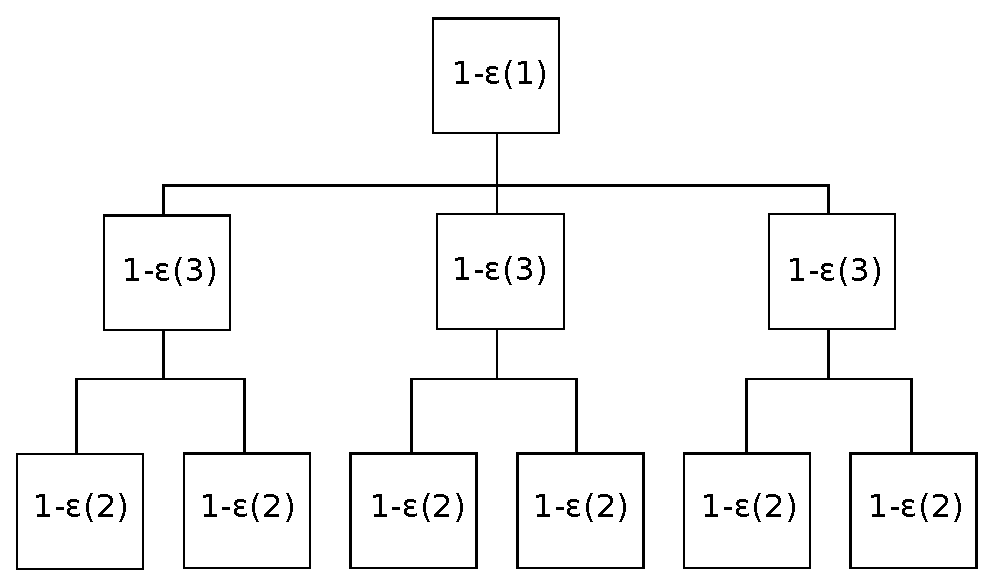
\includegraphics[width=\textwidth,draft=false]{images/effort.eps}
\includegraphics[width=\textwidth,draft=false]{images/effort2.eps}
\caption{\label{effort} \footnotesize\textbf{Mean field tree} - The Minimal Effort model estimates the effort necessary to build a graph as the sum of the cost of each node. }
\end{figure}
\newpage


\subsection{Minimizing the effort}
Despite the simplicity of the functional $\Ee$, it's not easy to make calculation keeping the whole complex structure of all possible trees. We need to simplify the topology.

Levels are labeled $\elle$, where the level $\elle=0$ correspond to the set of leaves and the level $\elle=\Elle$ is the set containing the root only. 
At each level $\elle$, the tree is essentially a set of nodes $\enne(\elle)$.

We can estimate the mean number of brothers that each node may have. It is given by the number of nodes at a level $\enne(\elle)$ divided by number of available parents, and so the number of nodes at successive level $\enne(\elle+1)$
\[ \emme(\elle) = \frac{\enne(\elle)}{\enne(\elle+1)} \]

Forgetting all details, let's consider a tree configuration all expressed by the number of nodes at each level, ignoring which nodes are linked together and which are not.
\[ \{ \enne(\elle) \}_{\elle=0}^{\Elle} = \{ \enne(0), \enne(1), \dots, \enne(\Elle)\equiv 1\} \]

With this simplification we can rewrite the effort as a sum over levels, and then
\[ \Ee [\Elle,\{ \enne(\elle) \}] = \sum_{\elle=0}^{\Elle-1} \left [ 1 - \varepsilon \left ( \frac{\enne(\elle)}{\enne(\elle+1)} \right ) \right ] \enne(\elle) \]
And expliciting the function $\varepsilon$ we obtain
\begin{equation}
\label{functional}
\Ee [\Elle,\{ \enne(\elle) \}] = \sum_{\elle=0}^{\Elle-1} \left ( 1 - e^{- \alpha \frac{\enne(\elle)}{\enne(\elle+1)}} \right ) \enne(\elle)
\end{equation}
 
It is now possible to obtain the minimum of the Effort $\Ee$ respect to the total number of levels $\Elle$ and the number of nodes at each level $\enne(\elle)$.
\[ \Ee^* = \min_{\Elle \, \{ \enne(\elle) \}} \Ee [\Elle,\{ \enne(\elle) \}]  \]

%------------------------%
\section{Numerical solutions}
Despite the lack of details about tree shapes, the model allows you the study of some important quantities, like nodes mean degree or population at each level. In this section results of numerical simulations about this quantities are shown for different parameters.

The minimization of the Effort functional \eqref{functional} has been made with the interior point method implemented in the program Wolfram Mathematica \cite{math}. The number of nodes, which is a discrete quantity by definition, is allowed to be real numbers in minimization process.

%---
\subsection{Finding optimal depth}
The Effort $\Ee$ is minimized respect to the number of nodes at each level $\{ \enne(\elle) \}$ and the depth $\Elle$, which is the maximum level accessible by the tree, that is populated by only one node, the root.

Free parameters of the model are $\enne(0)$, which is defined by the number of leaves, or the number of nodes necessary to solve the problem for which the tree has been created, and $\alpha$ which represents the abstractability.

Fixing reasonably values for these parameters, as $\enne(0)=1000$ and $\alpha=0.1$, we can look for the optimal depth $\Elle^*$ which minimize $\Ee$.
%
\begin{figure}[ht]%
\includegraphics[width=\textwidth,draft=false]{grafici/effVSdepth.1000.1.eps}
\caption{\label{FeffVSdepth} \footnotesize\textbf{The Effort as a function of depth} - When $\alpha=0.1$ and $\enne(0)=1000$, simulations show that the Effort is minimal for $\Elle=10$.}
\end{figure}

The numerical solution leads to $\Elle^*=10$, as showed in figure \ref{FeffVSdepth}.

%--
\subsubsection{Population at each level}
When the depth is optimal, the number of nodes is exponential in its dependence from the level, as shown in figure \ref{FpopVSlevdepth}.

Starting from a depth value lower than the optimal one and increasing it, the function representing the population at each level increases, approaching gradually the exponential function.

When optimal tree is reached, a further depth increase is ineffective to modify significantly the Effort value. The tree structure changes with the depth increase, but only near the optimal depth. When this point is exceeded of two units, the tree structure remains substantially unchanged and the only effect of depth increase is the addition of a node at the top of the graph, and so the addition of a new root linked to the old one only.

%--
\subsubsection{Outdegree mean}
Simulations of the function $\emme(\elle)$ reveal the behavioral change in population distribution respect to fixed depth. 

The ratio between the number of nodes of two consecutive levels is always increasing with levels until the optimal depth is reached. Then this quantity tends to be decreasing with levels, as shown in figure \ref{FpopVSlevdepth}.

This behavior is telling us that the effort is minimized when the outdegree mean is substantially constant with levels.

While number of nodes are allowed to be real number, levels are discrete quantities. We can then suppose that the minimum of functional $\Ee$ is somewhere between $\Elle =10$ and $\Elle =11$.

\begin{figure}[p]%
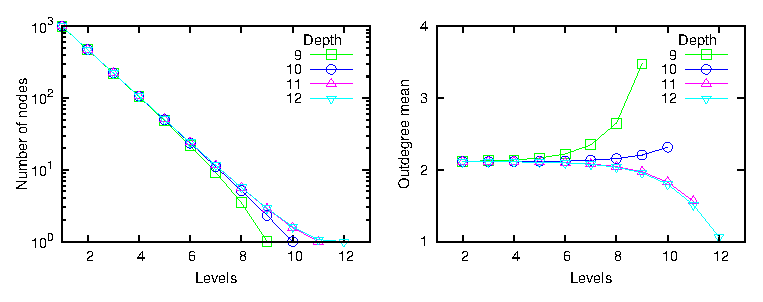
\includegraphics[width=\textwidth,draft=false]{grafici/Mdepth.eps}
\caption{\label{FpopVSlevdepth} \footnotesize\textbf{Distribution of nodes and outdegree mean for different values of depth} - When the depth is optimal, $\Elle=10$, nodes distribution is exponential, as showed in the left hand side figure. The right hand side shows that the optimal depth is the one for which outdegree vary as less as possible with levels. The costant function is often non accessible due to the fact that levels are discretized.}
\vspace{1cm}
\includegraphics[width=\textwidth,draft=false]{grafici/Mnodes.eps}%$y(x) = x*0.526328(+/- 0.0002096) + 2.10748 (+/- 0.7746)$
\caption{\label{FleaVSnod} \footnotesize\textbf{Leaves and nodes of optimal trees} - The figure on the left hand side shows that the dependence between total nodes and fixed initial leaves is linear. The linear fit leads to $y(x) \sim x/2 + 2$. At the right hand side, populations of nodes at each level of optimal depth for different values of leaves.}
\end{figure}

%---
\subsection{Varying number of leaves}
In order to complete this analysis, we have to study how results change varying the fixed initial parameters.  In this section, the abstractability is fixed $\alpha=0.1$.

The parameter $\enne(0)$ is the one which governs the total number of nodes of the tree. The dependence between nodes and leaves is linear, while the number of nodes is an exponential function of nodes for optimal trees, as showed in \ref{FleaVSnod}. There is a small deviation caused by the discrete nature of levels, that is visible when the level approaches the root.

The optimal depth, the one which minimizes the Effort, moves with the number of leaves. The minimum grows while the number of leaves $\enne(0)$ grows too. The dependence is almost linear, discretized by levels, as showed in \ref{FeffVSdepleaves} at the left hand side.

Keeping $\alpha=0.1$ fixed, and moving the number of leaves, we can observe the particular behavior of the outdegree mean as a function of levels showed at the right hand side of figure \ref{FeffVSdepleaves}. The optimal tree is the one whose outdegree mean is constant respect to levels. When the constant function is not accessible, the nearest function is chosen as optimal. This is the reason for which the derivative of outdegree respect to levels is oscillatory as a function of number of leaves.
\begin{figure}[p]%
\includegraphics[width=\textwidth,draft=false]{grafici/Mvarleaves.eps}
\caption{\label{FeffVSdepleaves} \footnotesize\textbf{Optimal depth and outdegree mean for different values of leaves} - The optimal depth increases with the number of leaves as $y(x) \sim x/1000 + 9$. At the right hand side, the outdegree mean as a function of levels for optimal depth.}
\vspace{1cm}
\includegraphics[width=\textwidth,draft=false]{grafici/Mvaralpha.eps}
\caption{\label{FeffVSdepalpha} \footnotesize\textbf{Optimal depth and outdegree mean for different values of $\boldsymbol{\alpha}$} - The optimal depth decreases with the number of leaves as $y(x) \sim 11 - 10x$. At the right hand side, the outdegree mean as a function of levels for optimal depth.}
\end{figure}

%---
\subsection{Varying abstractability $\alpha$}
The parameter $\alpha$ quantifies the portion of code that can be abstracted in higher levels, and so it represents the number of lines that nodes hold in common. In this section, the number of leaves is fixed $\enne(0)=1000$.

Numerical simulations show that if $\alpha$ is high, the optimal depth is low and vice versa. The position of the minimal Effort respect to depth moves linearly with $\alpha$, as showed in the left hand side of figure \ref{FeffVSdepalpha}.

The outdegree mean increses with $\alpha$, while its derivative remains oscillatory due to discrete levels. See figure \ref{FeffVSdepalpha}.
%



%******************************************************************************************************************************
\newpage
\clearpage{\pagestyle{empty}\cleardoublepage}
\newpage
\chapter{Sharing Tree model}
	\label{CTree}
%******************************************************************************************************************************
The Minimal Effort model is a \textit{mean field model}, needful to capture interesting behaviors in object-oriented programming. In addition, it is useful to introduce a \textit{microscopic model}, the Sharing tree model, which gives you a method to create inheritance structures and so which allows the construction of Monte Carlo trees, for data comparisons.

%%%%%%%%%%%%%%%%%%%%%%%%%%%%%%%%%%%%%%%%%%%%%%%%%%%%%%%%%%%%%%%%%%%%%%%%%%%%%
\section{Random objects}
Our starting point is a set of $\Enne$ classes which represents the computer science solution of a given problem. 

Consider each class composed by a set of different symbols randomly extracted from an alphabet. While the alphabet represents the whole writable code, each symbol represents a unit of code, as in the mean field model.

Each class is composed by a set of $\kappa$ symbols, and there are $\Esse$ symbols equally likely in the alphabet. This is a first approximation that allows you to find analytic results, but in principle not all units of code are equally important and used and not all classes have the same size.

The metric to measure the size of a code is an open question. The most popular method is \textit{counting source line of code}, subgrouped in physical lines (the whole code) and logical lines (the number of statements), but it is not necessarily an honest method. The same task can be performed by two different programs of different sizes and with different statements and you cannot know in advance whether the best program is the largest or the smallest.

A reasonable starting point is to consider classes of the same size, represented by $\kappa$, and a simplified alphabet where the $\Esse$ symbols are equally likely.

\begin{figure}[p]%
\center
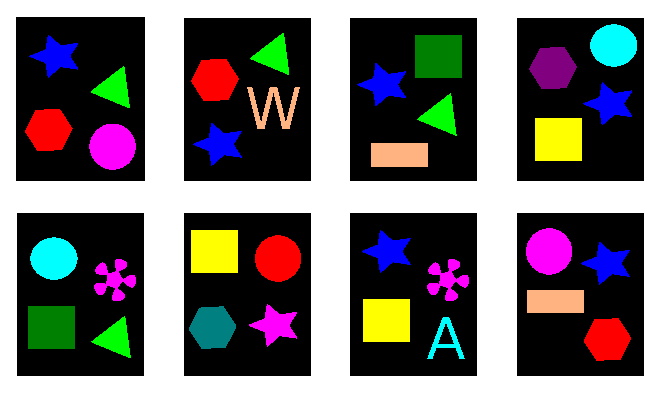
\includegraphics[width=7cm,draft=false]{images/sequenze.eps}
\caption{\label{Sequenza} \footnotesize\textbf{Example of initial sets} - In this $\Enne=8$ classes, only $\enne=6$ contain the most common symbol, the blue star.}
\vspace{2cm}
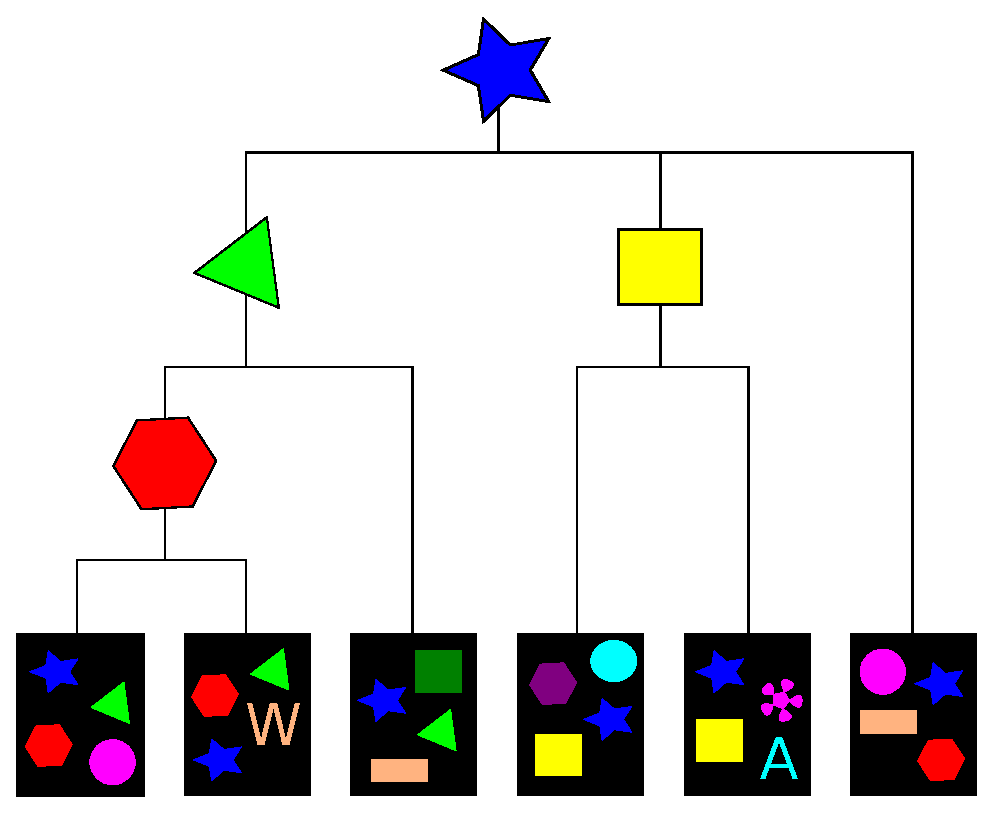
\includegraphics[width=\textwidth,draft=false]{images/sharingtree.eps}
\caption{\label{Albero} \footnotesize\textbf{Sharing Tree} - The most common symbol rule allows the creation of a tree. The $\enne$ classes represent the leaves, while each symbol chosen as the most common represents an internal node.}
\end{figure}

\section{Building the structure}
Once selected the $\Enne$ classes, rules are necessary to decide the structure of the tree. And so, how can we group classes in order to build a tree structure?

First, select the symbol that appears more often in the $\Enne$ classes. Keep classes with this symbol and delete the others. This symbol will be our root, and so the part of the code that all nodes of our tree hold in common. With the excluded classes one can in principle constructs other trees, but for now let just delete them.

The next step is the selection of the symbol that appears more often in the remaining $\enne$ classes. This symbol represents the second node of the tree, connected to the root only, for now.  

If $j$ classes contain this second symbol, we need to find the most common symbol in the $\enne-j$ remaining classes. The symbol is the third node, connected to the root. This process is iterated for all remaining classes until clustering is finished. The most common symbol groups all the classes in sets composed by different elements and with different number of element in each group. Furthermore, sets of one class are allowed: they are reminders of groupment, appearing once or even more times if the reminder is composed of more classes that hold nothing in common and for which the most common symbol rule does not work.

Each symbol used to group classes represents a node connected to the root, but it represents also a set of classes that have been grouped with such symbol.

When a group contains a single class, it means that its process is finished, but for each group with two or more classes the process can be iterated. The number of iterations necessary to finally arrive to all sets of one class only is $\Elle$, and it is exactly the depth of the tree. In fact, each step increases tree depth by one while it decreases the available symbols and the elements of each class by one (for this reason, $\kappa$ cannot be too small!).

Therefore, the process is finished when no group contains more than one class or when classes have no more symbols to be shared.

%%%%%%%%%%%%%%%%%%%%%%%%%%%%%%%%%%%%%%%%%%%%%%%%%%%%%%%%%%%%%%%%%%%%%%%%%%%%%%%%%%%%%%
\section{Most common symbol}
The key concept underlying the mechanism that grows trees from classes is the \textit{most common symbol rule}. Selecting the symbol that appears more often, we are applying an optimization principle: we are not interested in a random groupage, but in the best groupage in a certain defined sense.

It is not trivial to describe how the most common symbol is distributed, but with some calculations we can obtain lots of interesting results that substantially solve the model.

Then, to be quantitatively and to find analytical solutions we must find the answer to a probabilistic question: what is the occurrence of the most common symbol in $\Enne$ sets of $\kappa$ draws from an alphabet of $\Esse$ symbols without replacement?

The answer to this question is central for the model. Each groupage done to build the tree, follows the very same most common symbol rule. The analytic solution that we are looking for can be applied iteratively (with opportune parameters) in order to describe the distribution of the number of classes in each set and at each step. In a certain number of steps, sets become singletons and the process is over.

\subsection{Find a symbol in a sequence}
Unlike the choice made in the Minimal Effort model, Sharing Tree model symbols cannot be repeated in a sequence. Such refinement simplifies the following calculation but it also approaches the model to real classes in which code repetition does not have a well defined sense.

Thus, the probability to find a selected symbol in a sequence is given by the hypergeometric distribution
\[ p = \frac{\binom{\Esse-1}{\kappa-1}}{\binom{\Esse}{\kappa}}= \frac{\kappa!(\Esse -1)!}{\Esse!(\kappa -1)!} \]

\subsection{How many classes for each symbol?}
In how many classes does such symbol appear? The answer is given by the Binomial distribution of $\Enne$ trials in which the symbol can appear or not with probability $p$.

The Binomial distribution then describes the occurrence $w$ of each symbol in the $\Enne$ sequences. We can compute the probability that $w$ classes contain a selected symbol with
\[ Pr(w) = \binom{\Enne}{w} \, p^{w} \, (1-p)^{\Enne-w} \]

\subsection{What about the most common symbol?}
In the Sharing tree model, optimization is carried by the choice of the most common symbol, and not any one of them.

Let's say that each symbol $s \in \Esse$ appears in $w_s$ classes. The set $\{w_s\}_{s=1}^{\Esse}$ contains $\Esse$ random variables independent and identically distributed, and the most common symbol is the one that appears $\omega$ times
\[ \omega = \max \left\{ w_1, \dots, w_{\Esse} \right\} \]

In order to find the distribution of the occurrence of the most common symbol, it is necessary to do some calculations. Therefore, consider the cumulative distribution function of $\omega$
\[ F_{\omega} (y)= Pr(\omega \leq y) \]
Since $\omega$ is the maximal occurrence and the $w_s$ are independent, it holds that
\begin{align*}
Pr(\omega \leq y) &= Pr(w_1 \leq y, w_2 \leq y, \dots, w_{\Esse} \leq y) \\
&= Pr(w_1 \leq y) Pr(w_2 \leq y) \dots Pr(w_{\Esse} \leq y)
\end{align*}
and since all $w_s$ have the same cumulative mass function, we can write
\[ F_{\omega} (y) = F_{w}^{\Esse} (y) \]

The probability distribution of $\omega$ can now be obtained as the probability that $\omega \leq y$ minus the probability that $\omega \leq y-1$, and so
\begin{align*}
Pr (y = \omega) &= Pr (\omega \leq y) - Pr (\omega \leq y-1) \\
&= F_w^{\Esse} (y) - F_w^{\Esse} (y-1)
\end{align*}

\subsection{Probability distribution of most common symbol}
The occurrence of the most common symbol now is straightforward. Remembering that $w_s$ are binomial random variables, the occurrence $\omega$ of the most common symbol is therefore distributed as 
\[\Psi (\omega) = \left( \sum_{i=0}^{ \omega} \text{Bin}(\Enne, i) \right)^{\Esse}- \left( \sum_{i=0}^{\omega -1} \text{Bin}(\Enne, i) \right)^{\Esse}\]

Making explicit the formula of the Binomial distribution, we have finally obtained the distribution of the occurrence of the most common symbol
\[\Psi (\omega) = \left( \sum_{i=0}^{ \omega} \binom{\Enne}{i} p^i (1-p)^{\Enne -i} \right) ^{\Esse}- \left( \sum_{i=0}^{\omega -1} \binom{\Enne}{i} p^i (1-p)^{\Enne -i}\right) ^{\Esse} \]

Examples of this distribution for different parameters are shown in figures \ref{Tpsi1} and \ref{Tpsi2}.

\begin{figure}[p]%
\center
\includegraphics[width=\textwidth,draft=false]{grafici/campana1.eps}
\caption{\label{Tpsi1} \footnotesize\textbf{The function $\Psi (\omega)$ } - This figure represent the probability distribution of the occurrence of the most common symbol in $5000$ sequences of $100$ extracted symbols (without repetitions) from an alphabet of $2000$ symbols.}
\vspace{1cm}
\includegraphics[width=\textwidth,draft=false]{grafici/campana2.eps}
\caption{\label{Tpsi2} \footnotesize\textbf{$\Psi (\omega)$ for different parameters} - Some examples of the probability distribution of the occurrence of the most common symbol for different parameters.}
\end{figure}

\subsection{Mean occurrence of the most common symbol}
To make the calculations less demanding, often it is useful to deal with the mean instead of the whole distribution. We can obtain $\langle \omega \rangle$ expanding
\[ \langle \omega \rangle = \sum_{\omega = 1}^{\Enne} \omega \Psi(\omega) \]

To obtain the final simplified formula, some calculations are needed and in order to ease the notation, we can define $a_{\omega}$ as
\[a_{\omega} = \left( \sum_{i=0}^{ \omega} \binom{\Enne}{i} p^i (1-p)^{\Enne -i} \right) ^{\Esse} \]
and then rewrite $\Psi (\omega)$ as
\[\Psi (\omega) = a_{ \omega} - a_{ \omega-1} \]

Inserting the formula in the mean occurrence of the most common symbol, we have
\[\langle \omega \rangle = \sum_{\omega = 1}^{\Enne} \omega \left(a_{ \omega} - a_{ \omega-1}\right) \]
which is a telescopic series, that allows an important simplification 
\begin{align*}
\langle \omega \rangle &= 1\left(a_{1} - a_{0}\right) + 2\left(a_{2} - a_{1}\right)+ \dots + \Enne\left(a_{\Enne} - a_{\Enne-1}\right) \\
&= \Enne a_{\Enne} - a_{0} - a_{1} - \dots - a_{\Enne-1}
\end{align*}
Furthermore, considering that $a_{\Enne}$ is the sum over all possible cases of a probability, it is equal to $1$. Then we finally obtain
\[ \langle \omega \rangle = \Enne - \sum_{j=0}^{\Enne -1} a_j \]

Thus, the mean of the distribution of the occurrence of the most common symbol is explicitly
\[ \langle \omega \rangle =  \Enne - \sum_{j=0}^{\Enne -1} \left( \sum_{k=0}^{j} \binom{N}{k} p^k (1-p)^{\Enne -k} \right)^\Esse \]

With this formula, we can study directly how parameters change the mean of the number of leaves (but not of total nodes) of simulated trees, as shown in figure \ref{TwN}. Considering that, at each step, the groupage of classes in the process is made with the same rule, the formula for $\langle \omega \rangle$ can be applied iteratively to find the mean of the number of classes in each set and for each step of the recursive groupage.

\begin{figure}[p]%
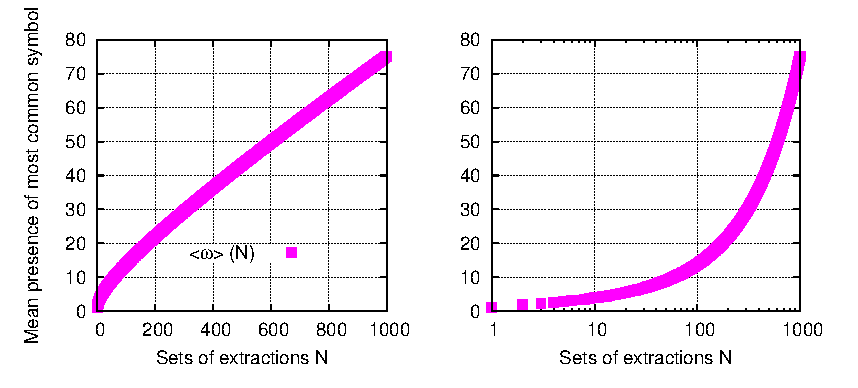
\includegraphics[width=\textwidth,draft=false]{grafici/meanN.eps}
\includegraphics[width=\textwidth,draft=false]{grafici/meank.eps}
\includegraphics[width=\textwidth,draft=false]{grafici/meanS.eps}
\caption{\label{TwN} \footnotesize\textbf{The mean occurrence $\langle\omega\rangle$ } - In the first figure, $\Esse$ and $\kappa$ are fixed at $\Esse = 2000$ and $\kappa = 100$ while and $\langle\omega\rangle$ is plotted as a function of $\Enne$. In the second figure $\Enne =500$ and $\Esse=2000$. In the third one, $\Enne=500$ and $\kappa=50$.}
\end{figure}

\section{Sharing process}
The recipe to build the tree can be seen also as the set of rules defining a process.

At each step, the recipe suggest to look for the symbol that appear more often and to group classes inspired by \textit{most common symbol rule}.

Following the iteration, the number of nodes are $ x_0 = \Enne, x_1, \dots , x_{\Elle} = 1$. Every time we divide classes in \textit{with} or \textit{without} the most common symbol, the process generate $\eta$ subprocesses, with $\eta$ the minimum number of subgroups necessary to cover all available classes.

Consider only the main process, which starts from $\Enne$ classes and which divides them into 2 subgroups, iteratively until the $x_{\Elle}$ is reached. All other subprocesses behave in the same manner with the opportune initial condition.

The mean number of elements of a group at each step $t$ is given by
\[ f(x_t, t) = x_t - \sum_{j=0}^{x_t-1} \left( \sum_{i=0}^{j} \binom{x_t}{i} \Pi_t^i \left( 1 - \Pi_t \right)^{x_t-i} \right)^{\Esse-t} \]
where $\Pi_t$ is obtained with the hypergeometric distribution and considering that if a symbol has been used as \textit{the most common} then it cannot be reused, and so at each step $\Esse \to \Esse -1$ and $\kappa \to \kappa -1$.
\[ \Pi_t = \frac{\binom{\Esse-1-t}{k-1-t}}{\binom{\Esse-t}{\kappa-t}} = \frac{\Gamma(\Esse-t)\Gamma(\kappa-t+1)}{\Gamma(\kappa-t)\Gamma(\Esse-t+1)}\]

The process for the mean number of elements can so be defined as
\[ x_{t+1} = f(x_{t},t) \]
where $x_0=x(0)$ and is equal to $\Enne$ for the main process.
%The initial condition is defined by the number of available classes, $x_0 = \Enne$.
%
\comment{
%\section{Alphabet and drawings}
%We need $\kappa\enne$ extraction. We can choose $\kappa$ and $\Esse$ with $\kappa < \Esse$ and then $\enne$ satisfying 
%\[ Z(\Esse) = \sum_{i=0}^{\Esse-1} \frac{\Esse}{\Esse-i} = \Esse\left (1+\frac{1}{2}+\frac{1}{3}+\dots+\frac{1}{\Esse} \right ) \]
%so that extractions are more then the mean minimum number necessary to span all the alphabet.
%If $\kappa\enne > Z(\Esse)$, all the alphabet is spanned.
%\begin{figure}[ht]%
%\center
%\includegraphics[width=9cm,draft=false]{grafici/wdiesse.eps}
%\caption{\label{Tesse} \footnotesize\textbf{The function Z(S)} }
%\end{figure}
}
%%%%%%%%%%%%%%%%%%%%%%%%%%%%%%%%%%%%%%%%%%%%%%%%%%%%%%%%%%%%%%%%%%%%%%%%%%%%%%%%%%%%%%%%%%%%%%%%%%
\section{Monte Carlo simulations}
What kinds of trees arise from Sharing Tree Monte Carlo simulations? To give an answer to this question, I have written a C++ code and I have integrated it with the data analysis library. The program is well optimized and fast and each tree is obtained in few seconds or less for all parameters that have been chosen.

In this section the simulations and the study of the behavior of trees are presented for different parameters.

\begin{figure}[p]%
\includegraphics[width=\textwidth,draft=false]{grafici/Tnodes.eps}
\caption{\label{Tnodi} \footnotesize\textbf{Initial nodes and number of leaves} - The mean number of leaves is a linear function of the initial number of nodes. The fit leads to $y=0.06x + 18$ when $k=100$ and $S=2000$. The function $\Psi (\omega)$ explains perfectly the leaves distribution.}
\vspace{1cm}
\includegraphics[width=\textwidth,draft=false]{grafici/Ttotnodes.eps}
\caption{\label{Ttotnodes} \footnotesize\textbf{Total nodes for different initial nodes} - While the distribution of total nodes is spread, its mean is linear in the number of initial nodes, with $y=0.2x + 58.7$ when $k=100$ and $S=2000$.}
\end{figure}

%------------------------
\subsection{Initial nodes and leaves}
This model does not allow you to fix the number of leaves of a tree, but only the number of initial nodes, among which leaves will be selected. Once fixed the $\Enne$ initial nodes, the tree will be built with a number of leaves whose dependence from this parameter has been obtained in the previous section and showed in figure \ref{TwN}.

In the range in which simulations were made, the mean number of leaves $\enne$ is substantially linear respect to the number of initial nodes $\Enne$, as shown on the left hand side of figure \ref{Tnodi}. This means that we can easily decide the mean number of leaves of simulated trees multiplying the number of initial nodes by the factor obtained from the linear fit.

The simulated distribution perfectly matches the analytic solution for the distribution of the most common symbol, as shown on the right hand side of figure \ref{Tnodi}, where the function $\Psi (\omega)$ exactly overlap the distribution of the number of leaves once fixed $\Enne$, $\Esse$ and $\kappa$.

%------------------------
\subsection{Total number of nodes}
The number of nodes in a tree consists in the number of leaves increased by the number of symbols used by the process. Due to the random nature of the number of leaves, the total number of nodes in a tree is usually a spread distribution.

Anyway, the mean is a linear function of the initial nodes and this allows to easily control the mean number of nodes of trees.

%------------------------
\subsection{Trees depth}
The depth $\Elle$ represents the number of steps in which all sets of classes, or sequences, have become singletons. In simulations, it has a sharp distribution, as showed on the right hand side of figure \ref{Tdepth}.

It is not surprising, since the number of classes in sets is strongly suppressed by each step of the process, with a small variance that decreases as a function of the number of classes, as deducible from figures \ref{TwN} and \ref{Tpsi2}.

The mean depth is a logarithmic function of initial nodes, as shown on the left hand side of figure \ref{Tdepth}. Since initial nodes are a linear function of total nodes, the logarithmic behavior of the depth is exactly the same result obtained from the Minimal Effort model. This is an optimal behavior for comparisons with data.

\begin{figure}[p]%
\includegraphics[width=\textwidth,draft=false]{grafici/Tdepth.eps}
\caption{\label{Tdepth} \footnotesize\textbf{Depth for different initial nodes} - Depth of trees has a sharp distribution, and the mean is a logarithmic function of the initial nodes, as $y=1.1\log(x) + 6.6$.}
\vspace{1cm}
\includegraphics[width=\textwidth,draft=false]{grafici/Toutdeg.eps}
\caption{\label{Toutdeg} \footnotesize\textbf{Outdegrees for different initial nodes} - The mean of outdegrees approaches $1$ for increasing number of initial nodes, while outdegrees distribution show a bizarre sharp peak for high outdegree.}
\end{figure}

%------------------------
\subsection{Outdegrees}
The outdegrees distribution shows an interesting behavior. While its mean approaches the value of $1$ for increasing number of initial nodes, as shown on the left hand side of figure \ref{Toutdeg}, the distribution of outdegrees is concentrated in low outdegree, but with a sharp peak of occurrence for high outdegree, as shown on the right hand side of \ref{Toutdeg}.

This means that some nodes share their code with lots of nodes, or in model terminology, that few symbols are used to group lots of nodes that have little more in common.

The gap in the distribution of outdegrees between the \textit{normal nodes} and \textit{special nodes} gradually becomes more and more pronounced while the number of initial node becomes higher, as detailed shown in figure \ref{TEoutdeg}.

This behavior can be investigated more closely studying the outdegree as a function of some variable, and this will be done in next section.

\begin{figure}[p]%
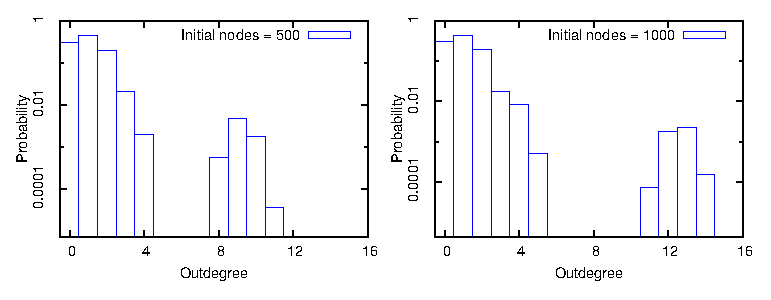
\includegraphics[width=\textwidth,draft=false]{grafici/TEXoutdeg1.eps}
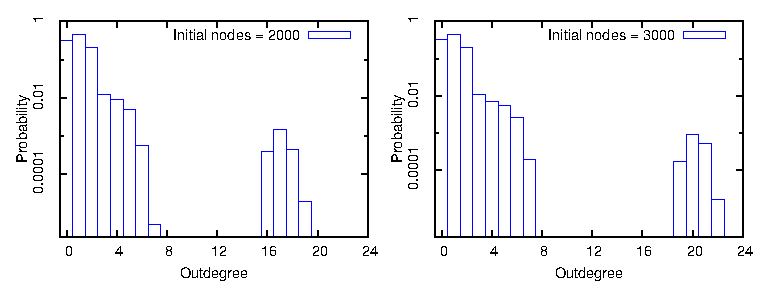
\includegraphics[width=\textwidth,draft=false]{grafici/TEXoutdeg2.eps}
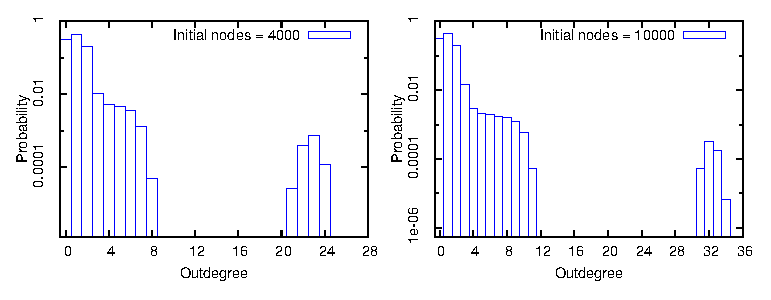
\includegraphics[width=\textwidth,draft=false]{grafici/TEXoutdeg3.eps}
\caption{\label{TEoutdeg} \footnotesize\textbf{Outdegrees distribution for different initial nodes} - The gap in the distribution of outdegrees becomes more and more pronounced while the number of initial node becomes higher.}
\end{figure}

%------------------------
\subsection{Outdegree mean per level}
A useful description of tree topology is the outdegree mean as a function of levels. In the Minimal Effort model we have seen how this function couples with the depth and that it shows a growth close to the root, strong or weak depending on the depth of the tree.

The microscopic rules of the Sharing Tree model lead to a very similar behavior. As shown on the top of figure \ref{Koutlev}, simulations build trees with an outdegree mean which grows with levels and which has a strong growth near the root.

Parameters govern the position and the height of peaks. In the bottom of figure \ref{Koutlev}, $\kappa$ and $\Esse$ are fixed, while $\Enne$ varies. The increase of the number of initial nodes moves the peak, and the depth, to higher levels and to higher outdegrees mean. More nodes need to been grouped, but they does not have many symbols in common.

On the top of figure \ref{KKoutlev}, the varying parameter is $\kappa$. When $\kappa$ is small, the depth is small since few symbols are available for groupage. When $\kappa$ grows, the height of the peaks does not change since it is coupled only with the number of leaves, and so with the number of initial nodes.

On the bottom of figure \ref{KKoutlev}, $\Esse$ is varying. The depth change with $\Esse$ and peaks move slowly while the number of possible symbols in $\Esse$ increases.

The behavior of outdegree mean as a function of level can be changed through the probability of each symbol in the alphabet. In this chapter, all symbols in alphabet are equally likely, but if some symbols would have more probability to be chosen in the extractions respect the others, we may expect a decline of peaks for higher depths. If there are few symbols with which we can initially group classes, then the outdegree mean of high levels will be lower, at least for one level. This argument will be useful in data analysis.

\begin{figure}[p]%
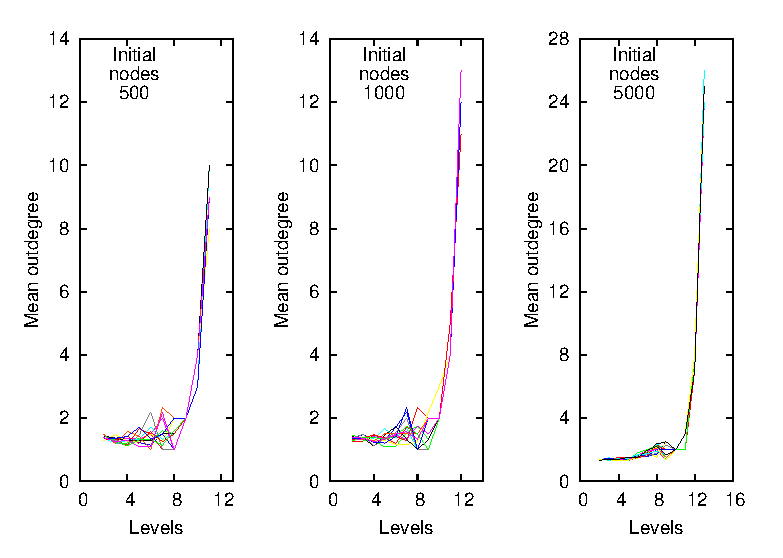
\includegraphics[width=\textwidth,draft=false]{grafici/ToutVSlev.eps}
\includegraphics[width=\textwidth,draft=false]{grafici/VoutVSlev3.eps}
\caption{\label{Koutlev} \footnotesize\textbf{Outdegree mean per level} - On the top, the figure shows some examples of outdegree mean as a function of levels for different initial nodes and with fixed depth. The figure on the bottom shows how the parameter $\Enne$ can change the simulated trees.}
\end{figure}

\begin{figure}[p]%
\includegraphics[width=\textwidth,draft=false]{grafici/VoutVSlev.eps}
\includegraphics[width=\textwidth,draft=false]{grafici/VoutVSlev2.eps}
\caption{\label{KKoutlev} \footnotesize\textbf{Outdegree mean per level} - Figures shows how parameters move the main quantities in simulated trees, as the depth and outdegrees distribution.}
\end{figure}


%******************************************************************************************************************************
\newpage
\clearpage{\pagestyle{empty}\cleardoublepage}
\newpage
\chapter{Data analysis}
	\label{Cdata}
%******************************************************************************************************************************
%\enlargethispage{\baselineskip}
How do programmer use inheritance? What kinds of graphs appear from hierarchical relations? In this chapter we analyze real hierarchical structures made by the Internet programmer community, among which appear users like Google, Facebook, Twitter and Microsoft \cite{gitwir}.
%******************************************************************************************************************************
\section{Dataset}
The dataset is composed by a huge amount of projects downloaded from GitHub, the actual largest code host on the web \cite{gitworld}. GitHub offers to its over 9.1 millions users \cite{gitpac}, source code management (directly from the program Git \cite{git}) which allows a cooperative programming among all users.

Inheritance hierarchies have been obtained directly from packages through different steps and with a particular attention to possible data bias and programs bugs.

\subsection{10 millions of hierarchies}
Packages have been downloaded in November 2014, and they have been chosen with a research by name (the whole alphabet) and by programming language (C++, Java, Python).

In detail, the dataset studied in this thesis contains:
\begin{itemize}
\item 17333 C++ projects (3233447 hierarchies)
\item 25318 Java projects (3504681 hierarchies)
\item 20010 Python projects (2491603 hierarchies)
\end{itemize}
Almost 10 millions of inheritance hierarchies!
\newpage
%\hskip10.5cm
\vphantom{cacca}
\vspace{3cm}
\begin{figure}[H]%
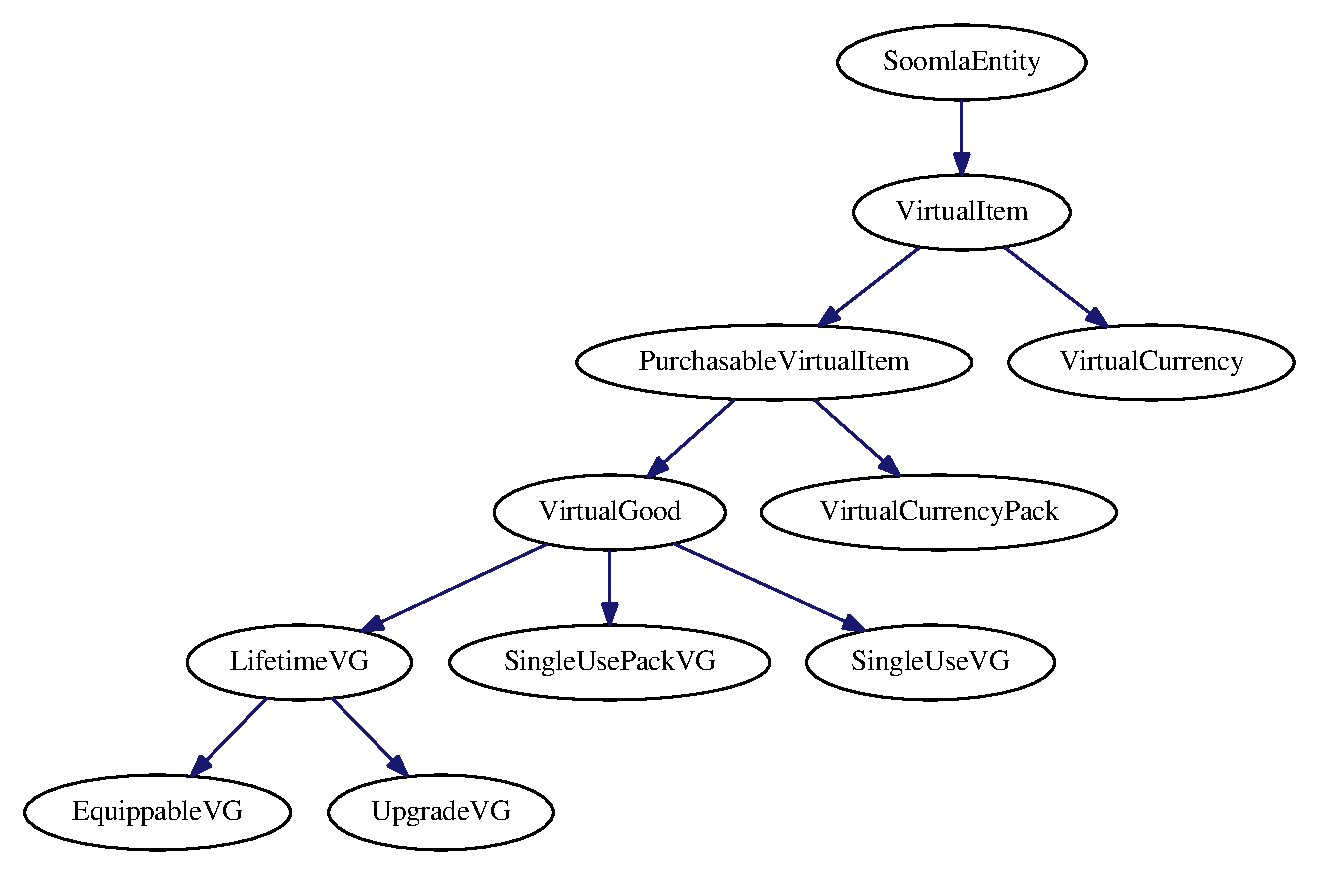
\includegraphics[width=\textwidth,draft=false]{images/soomla1.eps}
%\includegraphics[width=\textwidth,draft=false]{images/soomla4.eps}
%\caption{\label{gra1} \footnotesize\textbf{Distribution of the number of nodes in hierarchies} - The number of nodes composing the graphs has a power law distribution. The exponent $\sim x^{-2}$ is universal despite differences between the three languages.}
%\vspace{1cm}
%\includegraphics[width=\textwidth,draft=false]{images/soomla2.eps}
\caption{\label{gra1} \footnotesize\textbf{Example of hierarchical inheritance structure} - This is one of the graphs contained in the project Soomla Cocos2dx.}
\end{figure}
\newpage

\subsection{Data conversion}
Hierarchies reconstruction have been done by a series of scripts (see \ref{app} for examples) and with the aid of Doxygen \cite{doxy}, a program for code documentation.

Doxygen is not written with the goal of reconstructing inheritance hierarchies, but it gives you the chance of obtaining, for each class, a graph which reconstructs the hierarchy of the class \textit{upward} (any sister-classes are not included in graph). Cutting and pasting all the pieces of graphs, one can rebuild the whole hierarchy. This step has been done with the aid of gvpr, an \textit{awk} \cite{awk} inspired programming language useful for graphs manipulation.

Once obtained the hierarchies in the standard graphs format (.dot), finally the data have been converted in adjacency lists.

To analyze adjacency lists I have written a C++ library (see \ref{libra}) that allows the characterization of graphs (to calculate depth, to find roots and leaves, to assign levels to each node, to find eventually nodes not connected, \dots) and allows to obtain all principal statistical quantities, distributions and scatterplots.

To complete the analysis, I have written some C and bash scripts and lots of Gnuplot scripts to graphical the representation of the results.

\subsection{Templates and bias}
Analyzing converted data I came across some problems about their structure and composition.

For example, Doxygen consider as inheritance even the relation among a template class and all instances of its template variable. Since I don't consider such relation as inheritance, I wrote a script to exclude fake links among classes.

The second important problem was about data redundancy. Due to the sharing nature of open source code, it often happens that some big libraries are contained in slightly different versions in many packages. I can't exclude all redundancy from data, but I made some general controls to exclude packages that caused the most obvious bias. Instead, I considered good packages those whose libraries are not comparable to the naked eye, since they contain information useful for my analysis.

%******************************************************************************************************************************
\begin{figure}[p]%
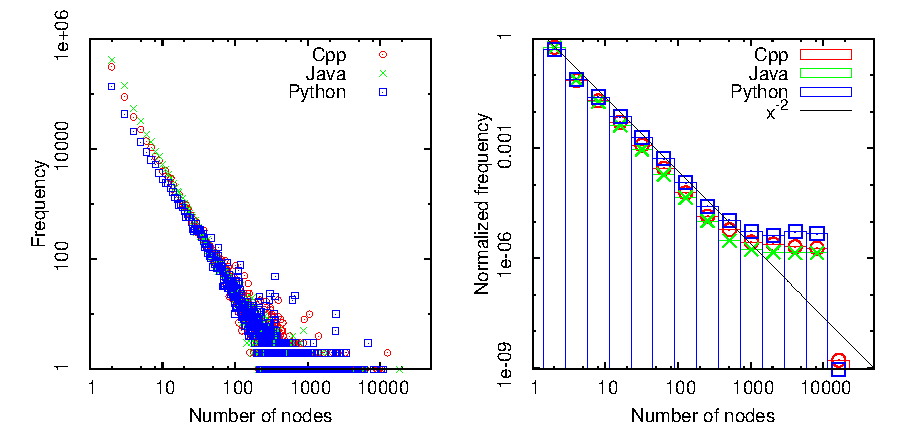
\includegraphics[width=\textwidth,draft=false]{grafici/fDNnodes.eps}
\caption{\label{Fnodes} \footnotesize\textbf{Distribution of the number of nodes in hierarchies} - The number of nodes composing the graphs has a power law distribution. The exponent $\sim x^{-2}$ is universal despite differences between the three languages.}
\vspace{1cm}
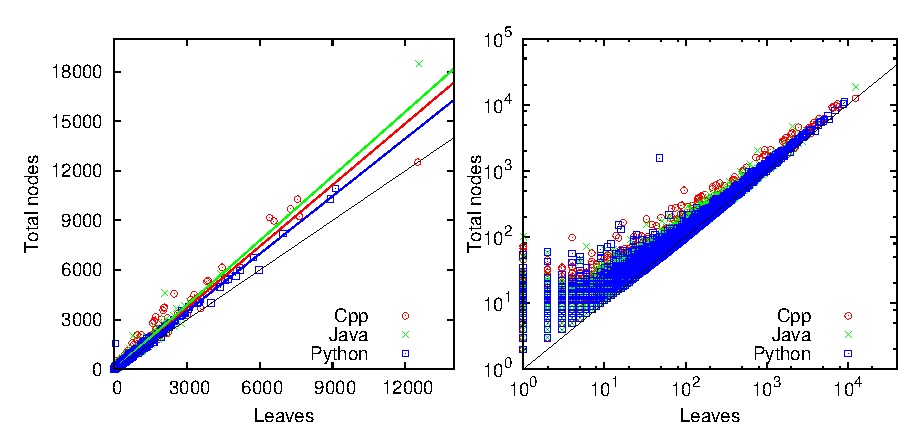
\includegraphics[width=\textwidth,draft=false]{grafici/leavesnodes.eps}
\caption{\label{Fleanodes} \footnotesize\textbf{Leaves and total nodes} - If a point (representing a graph) is near the black line, it means that almost all nodes of the graph are leaves, and so that only few nodes contain the shared code, while lots of classes inherit it.}
\end{figure}

\section{Graphs sizes}
The first important approach to noisy data is the sizes distribution. Graphs sizes and complexity is in some way coupled with the complexity of problems for which the whole set of programs is made for. In this thesis, I am not investigating the \textit{problems space}, that is true head of such distribution, but the whole following analysis will feel the consequences of sizes distribution.

The size of a directed acyclic graph can be defined in different ways. For our purposes, it is important to consider two main quantities: the number of nodes (and so of classes) which is the effective representation of hierarchy purpose, and the depth of graphs, which is the amount representing the hierarchies optimization.

\subsection{Solutions sizes}
Consider each hierarchy as the solution for a computer science problem, or task. How many classes are necessary to solve problems?

First of all, we analyze the total number of nodes of each graph (i.e. the number of classes of each hierarchy), the most important quantity to define the size of structures.

Plotting this quantity for each graph for each package, as showed in figure \ref{Fnodes}, we find a power law distribution with a small exponent ($\sim x^{-2}$).

Despite the differences among C++, Java and Python, this behavior is universal: hierarchies sizes are distributed in the same way, regardless the language in which they are built. This is the first interesting result that arise from the analysis: in principle, programming languages can be used to perform different tasks and they are designed in different ways and for different purposes. This seems not to influence the structure of inheritance hierarchies, at least in sizes distribution.

\begin{figure}[p]%
\includegraphics[width=\textwidth,draft=false]{grafici/fDdepth.eps}
\caption{\label{Fdepth} \footnotesize\textbf{Distribution of depth of each hierarchy} - While C++ and Python have the same power law distribution ($\sim x^{-5}$), Java structures are systematically less deeper than other languages.}
\vspace{1cm}
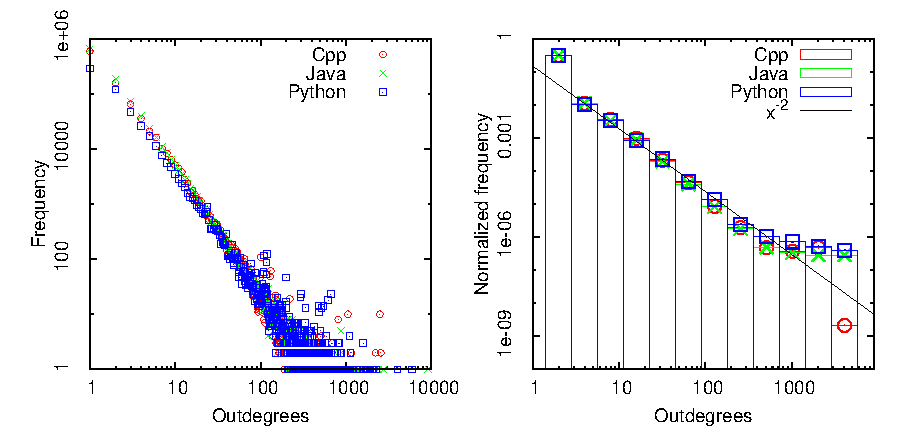
\includegraphics[width=\textwidth,draft=false]{grafici/fDoutdeg.eps}
\caption{\label{Foutdeg} \footnotesize\textbf{Distribution of outdegrees of all nodes of all graphs} - The outdegree quantifies the number of classes that inherits code from the same class. Its power law behavior can be caused by the power law distribution of the number of nodes of each graph, showed in figure \ref{Fnodes}. }
\end{figure}

\subsection{Sharing classes}
Not all classes of a hierarchy are directly used in programs: for example, abstract classes cannot be instantiated, and in general some classes can be built for sharing code purposes, abstracting concepts in \textit{super classes}.

While, in first approximation, we cannot know if an internal node is used or not, we can be sure that the leaves of each hierarchy are instantiable and that such classes are made to solve the task.

How many are the leaves compared to the total number of classes? How many classes share their code?

The answer is shown in figure \ref{Fleanodes}: the vast majority of classes in each hierarchy are leaves, i.e. classes that can be used in programs.

This result give us an important clue to argue that inheritance graphs take place only for high abstractability. If almost all nodes are leaves, as happens in the data, only few nodes are responsible of the collection of all the code that can be shared, while many nodes inherit it. The shared code must be useful for lots of classes, and lots of classes must hold something in common.

This behavior makes us also to think about a general small depth of graphs, and in next section we will check it.

\subsection{Depth of hierarchies}
Hierarchies depth is a surprisingly small quantity: also the largest structures have at most eleven or twelve levels, while the vast majority of graphs have a depth equal to two or three. This result is the second clue that supports the idea for which abstractability is high in all real hierarchies.

Another important result given by figure \ref{Fdepth} is that Java language does not behave as C++ and Python: depths distribution of Java hierarchies is consistently below the other two distributions. The reasons of this discrepancy can be found directly in Java inheritance implementation rules. In Java, multiple inheritance is allowed only by a special kind of relation given by the keywords \textit{interface} and \textit{implements}. \textit{Interface} is the kind of class that can be inherited without limitations about the multiple inheritance, but \textit{implements} is the keyword that the class which inherits the interface must have: an interface cannot contains \textit{implementation}, but only declarations of methods and functions. The reasons for which a class inherits from interfaces is code reuse as well, but not in the sense expressed by models in sections \ref{Ceffort} and \ref{CTree}.

This and other features have been inserted in Java language in order to obtain a simpler and more safe programming. We can expect other differences in data between Java and the other two languages. We can say that Java inheritance rules give rise to less deeper hierarchies respect to other languages (especially C++ from which Java is developed), and in this sense they have a simplified effect as hoped by Java designers.

%******************************************************************************************************************************
\begin{figure}[p]%
\includegraphics[width=\textwidth,draft=false]{grafici/fDindeg.eps}
\caption{\label{Findeg} \footnotesize\textbf{Distribution of indegrees of all nodes of all graphs} - Indegrees are systematically less than outdegrees and distributions have a strong cutoff, especially for Java hierarchies.}
\vspace{1cm}
\includegraphics[width=\textwidth,draft=false]{grafici/depVSNnodes.err.eps}
\caption{\label{FdVSnerr} \footnotesize\textbf{Depth VS Nnodes } - Depth of graphs seems a logarithmic function of the number of object for C++ and Python, while the depth is almost constant in Java hierarchies. The fit for C++ and Python give $y \sim 0.5\log(x)+1.5$}
\end{figure}

\section{Code shareability}
The outdegree quantifies the number of classes that inherit code from the same class. The power law distribution of graphs sizes affects outdegrees distribution (over all nodes of all graphs), which appears as a power law with the same exponent ($\sim x^{-2}$). This is not a surprising result, since regardless the outdegrees distribution of each graph, its sum over all graphs (which sizes are power law distributed) will have a power law shape as well. See figure \ref{Foutdeg}.

For this reason, it's important to look at outdegrees distribution of each graph. Is the outdegrees distribution a real power law or it is an effect caused by the sizes?

As showed in figure \ref{Finoutd}, the power law appears as distribution of outdegrees also in single graphs, at least for biggest hierarchies. Outdegrees distribution is therefore the results of the sum of many power laws.

%fare grafico con l'esponente della powerlaw dell'outdeg VS numero di nodi? sono tutte powerlaw davvero'
%******************************************************************************************************************************
\section{Tree approximation}
Models presented in sections \ref{CTree} and \ref{Ceffort} schematize hierarchies through trees, while inheritance structures can be in principle directed acyclic graphs. The main difference between this two kind of graphs is in the number of indegrees of each node: if a graph is a tree, all nodes can have at most one indegree, while indegrees have no restrictions for a directed acyclic graph.

In programming languages, multiple inheritance is often not recommended, except in cases where actually required. In data we can observe multiple inheritance, but it is systematically less than single inheritance, as expected. When indegrees distribution is compared to outdegrees distribution in a hierarchy, as in figure \ref{Finoutd}, one can observe how outdegree is the first main quantity to keep into account in an object-oriented hierarchy model.

The outdegrees distribution shows power law behavior with a small exponent ($\sim x^{-2}$ or even less), while indegrees distribution shows a power law behavior with a large exponent ($\sim x^{-3}$ and often more), large enough to allow a first approach considering the indegree constant and equal to its mean, that is about $1$. In this sense, tree approximation is an excellent first approach to this system.

Distribution of indegrees of all nodes of all graphs shows a power law behavior, with exponent $\sim x^{-3}$ (see figure \ref{Findeg}). The three programming languages have quite different behaviors. In Python only the $0.1\%$ of nodes has outdegree greater than one and no one class has more than $300$ indegrees. In Java, indegrees are often more respect to other languages, as expected from an \textit{interfaces programming}, but all class has less than $100$ indegrees. In C++ indegrees can reach $1000$ classes.

\begin{figure}[p]%
\includegraphics[width=\textwidth,draft=false]{grafici/cppinout.eps}
\includegraphics[width=\textwidth,draft=false]{grafici/javainout.eps}
\includegraphics[width=\textwidth,draft=false]{grafici/pyinout.eps}
\caption{\label{Finoutd} \footnotesize\textbf{Comparison between indegrees and outdegrees} - The different exponent for indegree and outdegree in each graph shows how tree approximation is an excellent first approach to this system.}
\end{figure}

%******************************************************************************************************************************
\section{Lateral growth}
Graphs are complex structures and their topology has lots of features. A way to give a summary look into its shape is asking in which way the depth is coupled to the number of objects in hierarchies, in order to have an idea about the ratio of the \textit{vertical} dimension (i.e. the depth) and the \textit{horizontal} dimension (i.e. the number of objects in levels).

\subsection{Horizontal and vertical dimensions}
Plotting the depth versus the number of objects for each graph allow to reconstruct a distribution of occurrence for each programming language, which means and standard deviations are showed in figure \ref{FdVSnerr}.

Python and C++ behave in the same way: the depth is in good approximation a logarithmic function of the number of objects (at least for most of sizes). For Java hierarchies, instead, the depth is almost a constant function of the number of classes that grows only for big graphs sizes. Both results are descriptive of a \textit{later growth} of graphs instead of a vertical one.

Consider two hierarchies with a very different number of objects. Despite the gap between the two effective sizes of the structures, we may expect two graphs with similar depths, at most one increased or decreased by one respect the other, especially for Java structures.

The logarithmic behavior of the depth as a function of the number of objects is well captured by the Sharing Tree model and the Effort model. Both mean field hierarchies and simulated trees well describe this feature.

\subsection{Shallow is better}
A really interesting result is the change in behavior of the depth as a function of the number of objects, as highlight in figure \ref{FdVSnheat} through a heat map for each programming language. 

In object-oriented programming languages there are general advices that suggest to keep hierarchies as shallow as possible, in order to avoid the anti-pattern known as \textit{Yo-yo problem} \cite{yoyo}. If inheritance graph is too much long and complicated, then a programmer that has to read and understand the hierarchy, has to keep flipping between different parts of the code.

For these reasons, the huge amount of shallow hierarchies was foreseeable. But what happens when hierarchy size get over $1000$ classes?

The artificial attempt to keep hierarchies as shallow as possible seems to fail, and all hierarchies show a depth greater than that expected.

Can the guess for which \textit{shallow is better} be wrong? If shallow hierarchies are produced by a false assumption, can the optimization be achieved through deep hierarchies?

\begin{figure}[p]%
\includegraphics[width=\textwidth,draft=false]{grafici/Heatmap.cpp.eps}
\includegraphics[width=\textwidth,draft=false]{grafici/Heatmap.java.eps}
\includegraphics[width=\textwidth,draft=false]{grafici/Heatmap.py.eps}
\caption{\label{FdVSnheat} \footnotesize\textbf{Depth VS nodes in C++, Java and Python hierarchy} - Colors (used in log scale) are representative of how many graphs have the $x$ number of nodes and depth equal to $y$. Colors represent the whole distribution, while lines trace the mean. Comparison of this three trends is given in figure \ref{FdVSnerr}. }
\end{figure}

%******************************************************************************************************************************
\section{Vertical balancing}
Inspired by models, we can investigate more accurately the topology of hierarchies studying the behavior of the outdegree mean of nodes as a function of the levels. Is it constant across graphs? If not, where are situated objects with the most shared code?

\subsection{Code shareability per level}
Once established that graphs are wider than high, we can probe the \textit{vertical balancing}. An interesting quantity that we can study as a function of a vertical variable (i.e. of levels) is the outdegree mean of nodes.

When the outdegree is high, the code contained in classes is shared with lots of other classes: high outdegree means high shareability.

Some examples of this function are given in figures \ref{Foutdegcpp} and \ref{Foutdegjp}. We can observe that the outdegree mean is a quantity that tends to grow with levels, with pronounced peaks close to the root. 

Why this behavior? Why the outdegree mean grows with level?

\begin{figure}[ht]%
\includegraphics[width=\textwidth,draft=false]{grafici/Coutdeg.cpp2.eps}
\caption{\label{Foutdegcpp} \footnotesize\textbf{Outdegree mean for Cpp hierarchies} - Examples of structure with more than 1000 nodes and depth equal to 6, 7 and 8 (in order).}
\end{figure}

\begin{figure}[hp]%
\includegraphics[width=\textwidth,draft=false]{grafici/Coutdeg.java.eps}
\includegraphics[width=\textwidth,draft=false]{grafici/Coutdeg.py.eps}
\caption{\label{Foutdegjp} \footnotesize\textbf{Outdegree mean for Java and Python hierarchies} - In the upper side figures, examples of Java structure with more than 500 nodes and depth equal to 4, 5 and 6 (in order). The other figures represent examples of python structure with more than 500 nodes and depth equal to 6, 7 and 8 (in order).}
\end{figure}

\subsection{Shallow regime}
Thanks to the mean field model (Effort model), we can give an interpretation to the growth of outdegree with levels.

We have showed in chapter \ref{Ceffort} how the outdegree mean behavior, as function of levels, is very sensible to \textit{depth constrain} and that it can have a strong growth close to the root in the case of insufficient depth. This is exactly the situation in which we find inheritance hierarchies in data.

This is yet another clue that leads us to argue that \textit{shallow hierarchies} are not the best solution. Code reuse appears not optimized by a decrease of the depth in Effort model, and data appears as trapped in an artificial \textit{shallow regime}.

A most efficient documentation system could avoid the \textit{yo-yo problem} as well as decreasing the depth of hierarchies, without sacrificing the optimal depth.

%******************************************************************************************************************************
\section{Optimal or random?}
The models proposed in this thesis are based on the assumption that inheritance graphs are made with optimizing spirit. This is a perfectly reasonable assumption since there are no reasons to hypothesize that inheritance arise from chaos.

Anyway, it is interesting to compare Sharing Tree graphs with graphs obtained through models completely random and made without optimization mechanisms.

\subsection{Random Branching Tree model}
A Random Branching Tree can be built starting from an initial node, the root, and choosing a distribution with a well-defined mean.

As a first step, we extract a random variable from the distribution: the extraction represents the root outdegree and so the number of nodes that are connected to the root. Once added new nodes, the process is iterated for each new node until a certain condition is reached.

The outdegree mean in function of levels is obviously a constant value, equal to the mean of the chosen distribution for the outdegree. Simulations are shown in figure \ref{Foutrpm}.

Which random mechanism can be introduced to obtain a non constant function? 

\begin{figure}[p]%
\includegraphics[width=\textwidth,draft=false]{grafici/Coutdeg.yul.eps}
\includegraphics[width=\textwidth,draft=false]{grafici/Coutdeg.rus.eps}
\caption{\label{Foutrpm} \footnotesize\textbf{Random branching tree and Pang-Maslov models simulation} - The outdegree mean in function of levels does not reproduce the behavior observed in data.}
\end{figure}

\subsection{Pang-Maslov model}
The Pang-Maslov model \cite{pangmaslov} can be used to construct a tree. Consider an initial node an a process for which, at each step, a new node arrives and sticks to one of the existing nodes. The process can be iterated until a certain condition is reached.

This model prevents the constancy of outdegree mean, since the older nodes have had more chance of being chosen by another node, and so they must have an outdegree greater than young nodes. Growth, however, is constant and it does not represent well the behavior of outdegree mean in data.

\subsection{Sharing Tree comparison}
Through the Sharing Tree model, we can can produce Monte Carlo trees to explicitly compare optimization ideas with data. Some examples are given in figure \ref{STsim}.

The outdegree mean has not a trivial behavior due to its strong growth close to the root, that is also the main feature observable in data.

Therefore, there is a very good agreement between data and optimization models.

\begin{figure}[htp]%
\includegraphics[width=\textwidth,draft=false]{grafici/STsim.eps}
\caption{\label{STsim} \footnotesize\textbf{Sharing Tree Monte Carlo simulations} - The Sharing Tree model well capture the behave of the outdegree mean as function of levels. In simulations, parameters are $\Enne=1000$, $\kappa=100$ and $\Esse=2000$.}
\end{figure}


%******************************************************************************************************************************
\newpage
\clearpage{\pagestyle{empty}\cleardoublepage}
\newpage
\chapter{Conclusions}
%******************************************************************************************************************************
The noisy data have proved to be full of interesting information: they have showed universal behaviors among object-oriented programming languages but they also highlight structural differences in inheritance management.

%Models are useful allies in data analysis. The mean field model allows an interpretation 
%
\subsubsection{Hierarchical sizes distribution is universal}
%The scale-free power law seems to be the dominant distribution of every main quantity obtained from data and the exponents are almost universal.
Hierarchies sizes distribution is power law distributed and there are no differences among the three programming languages.

\subsubsection{The speciation of classes has a universal behavior}
Despite the differences among C++, Java and Python, the speciation is used in the same way, and so the distribution of the number of classes that inherits code from a selected class is the same.

\subsubsection{Multiple inheritance is ever less used than speciation}
The multiple inheritance is used with differences between the three languages. It is always used less than speciation, even in Java, where it has a different and more useful meaning.

\subsubsection{Hierarchies are shallow}
The vast majority of graphs have a depth equal to two or three while the deepest hierarchies have at most a depth of about eleven, or twelve.

\subsubsection{Java hierarchies are shallower}
Java hierarchies show a depth sistematically lower than the Python and C++, while graph sizes behave in the same way.

\subsubsection{The depth is a logarithmic function of the hierarchy size}
In C++ and Python, the mean of depths of hierarchies as a function of the number of classes has a logarithmic behavior.

\subsubsection{Huge hierarchies behave differently}
The depth of huge hierarchies doesn't fit the logarithmic behavior of small and medium hierarchies. It is systematically over such function.

\subsubsection{Speciation is a function of levels}
Classes that does lots of speciation are always at the higher levels.

\vspace{1cm}
The Minimal Effort model gives a link between the hierarchical structures and the effort done to build them. It allows to give an interpretation to data, and it is a guide to key quantities.

\vspace{0.5cm}
The Sharing Tree model extends the mean field model and allows Monte Carlo simulations. The mechanism implemented is close to the natural approach of programmers in objects organization and Sharing Monte Carlo trees well reproduce the data hierarchies.

\vspace{0.5cm}
The depth is the central quantity for optimization mechanism, since it governs the hierarchical structures for fixed size and the proportion between the vertical and the horizontal dimension. Programmers seems to follow the advise to keep the depth as shallow as possibile to avoid the yo-yo problem instead of looking for the optimal structure for code reuse.

\vspace{0.5cm}
The optimization resulting from the competition between the reuse and the abstractability of the code seems to play an important role in the construction of hierarchical inheritance structures in object-oriented programming languages.


\comment{
 caused by the different rules chosen by Java designers.

Java designers have obtained one of their proposals: Java hierarchies are sistematically shallow then C++ and Python ones.


Il numero di oggetti che compongono le strutture gerarchiche ha una
distribuzione a potenza, sostanzialmente universale rispetto ai tre linguaggi
di programmazione analizzati.


In particolare, il linguaggio di programmazione Java presenta strutture
sistematicamente meno profonde rispetto agli altri due linguaggi presentati.
Questo ed altri comportamenti anomali sono frutto di alcune importanti
differenze nella gestione dell’ereditariet`a decise dagli ideatori del linguaggio
Java e con l’obiettivo di minimizzare la complessit`a strutturale del codice,
obiettivo che grazie all’analisi dati possiamo dichiarare raggiunto sotto molti
aspetti.

L’osservazione critica dei dati attraverso le previsioni del modello mean
field propone un primo risultato interessante: le gerarchie appaiono meno
profonde di quelle ottimali. Nei dati si evince infatti che l’outdegree medio
`e generalmente una quantit`a decrescente come funzione della distanza dalla
radice, trend che viene interpretato dal modello come un regime non ottimale
a causa di una profondit`a troppo bassa. Questo risultato `e altres`ı confermato
da generali istruzioni che in ambito informatico suggeriscono di limitare la
complessit`a delle gerarchie in funzione di un pi`
u semplice utilizzo delle stesse.

La previsione dell’andamento dell’outdegree medio come funzione del-
la distanza dalla radice nel modello Sharing Tree risulta una funzione ben
sovrapponibile all’effettivo comportamento delle gerarchie nei linguaggi di
programmazione.

Altre quantit`a nei dati sono risultate in pieno accordo con i modelli,
come ad esempio la profondit`a delle strutture come funzione del numero di
oggetti della gerarchia che si presenta in buona approssimazione logaritmica,
comportamento previsto da entrambi i modelli.



%\begin{figure}[ht]%
%\includegraphics[width=\textwidth,draft=false]{grafici/Coutdeg.cpp1.eps}
%\caption{\label{Foutdeg} \footnotesize\textbf{Cpp} - Very beautiful.}
%\end{figure}


}

%******************************************************************************************************************************
\newpage
\clearpage{\pagestyle{empty}\cleardoublepage}
\newpage
\appendix
\chapter{Source code} 
%******************************************************************************************************************************
\section{Library for data analysis}
\label{libra}
In this section, some of the classes implemented in the library are listed. Classes omitted are Scatterplot, Lineplot and Distribuzioni that allow a suitable print of data obtainable by the following classes.

\subsection{class Node}
A class that realize the concept of node.
\subsubsection{node.hpp}
\lstinputlisting[language=C++,style=customc]{codice/libreria/node.hpp}
\vspace{0.5cm}
\subsubsection{node.cpp}
\lstinputlisting[language=C++,style=customc]{codice/libreria/node.cpp}
\vspace{0.5cm}

\subsection{class Graph}
The class Graph is central for the library. It allows to obtain all main quantities about a graph, or a tree.
\subsubsection{graph.hpp}
\lstinputlisting[language=C++,style=customc]{codice/libreria/graph.hpp}
\vspace{0.5cm}
\subsubsection{graph.cpp}
\lstinputlisting[language=C++,style=customc]{codice/libreria/graph.cpp}
\vspace{0.5cm}

\subsection{class Packagegraph}
This class is a tool that allows to analyze automatically more graphs at the same time.
\subsubsection{packagegraph.hpp}
\lstinputlisting[language=C++,style=customc]{codice/libreria/packagegraph.hpp}
\vspace{0.5cm}
\subsubsection{packagegraph.cpp}
\lstinputlisting[language=C++,style=customc]{codice/libreria/packagegraph.cpp}
\vspace{0.5cm}

\subsection{class Treemaker}
This class builds trees and graphs through Sharing Tree model, Pang-Maslov model and Branching Tree model.
\subsubsection{treemaker.hpp}
\lstinputlisting[language=C++,style=customc]{codice/libreria/treemaker.hpp}
\vspace{0.5cm}
\subsubsection{treemaker.cpp}
\lstinputlisting[language=C++,style=customc]{codice/libreria/treemaker.cpp}
\vspace{0.5cm}

\comment{
\subsection{class Distribuzioni}
This class calculates distributions about all main quantities in this analysis.
\subsubsection{distribuzioni.hpp}
\lstinputlisting[language=C++,style=customc]{codice/libreria/distribuzioni.hpp}
\vspace{0.5cm}
\subsubsection{distribuzioni.cpp}
\lstinputlisting[language=C++,style=customc]{codice/libreria/distribuzioni.cpp}
\vspace{0.5cm}

\subsection{class Scatterplot}
Scatterplots have a fundamental role in this analysis. This class allows to obtain all scatterplots contained in this thesis.
\subsubsection{scatterplot.hpp}
\lstinputlisting[language=C++,style=customc]{codice/libreria/scatterplot.hpp}
\vspace{0.5cm}
\subsubsection{scatterplot.cpp}
\lstinputlisting[language=C++,style=customc]{codice/libreria/scatterplot.cpp}
\vspace{0.5cm}

\subsection{class Lineplot}
While distributions and scatterplots are done for the whole dataset, the class Lineplot allows to obtain an analysis from each graph.
\subsubsection{treemaker.hpp}
\lstinputlisting[language=C++,style=customc]{codice/libreria/lineplot.hpp}
\vspace{0.5cm}
\subsubsection{treemaker.cpp}
\lstinputlisting[language=C++,style=customc]{codice/libreria/lineplot.cpp}
\vspace{0.5cm}

\subsection{Tools}
Miscellaneous tools for the library.
\subsubsection{funzioni.hpp}
\lstinputlisting[language=C++,style=customc]{codice/libreria/funzioni.hpp}
\vspace{0.5cm}
\subsubsection{funzioni.cpp}
\lstinputlisting[language=C++,style=customc]{codice/libreria/funzioni.cpp}
\vspace{0.5cm}
\subsubsection{libreria.hpp}
\lstinputlisting[language=C++,style=customc]{codice/libreria/libreria.hpp}
\vspace{0.5cm}
\subsubsection{Uniqa}
\lstinputlisting[language=bash,style=customc]{codice/programmi/Uniqa}
\vspace{0.5cm}
\subsubsection{Sorta}
\lstinputlisting[language=bash,style=customc]{codice/programmi/Sorta}
}

\section{Programs for simulations and analysis}

\subsection{mrmodel.cpp}
This program use the library to simulate and analyze Sharing Trees.
\lstinputlisting[language=C++,style=customc]{codice/libreria/mrmodel.cpp}
\vspace{0.5cm}

\subsection{tarantola.cpp}
A program to obtain the whole data analysis through the library.
\lstinputlisting[language=C++,style=customc]{codice/libreria/tarantola.cpp}
\vspace{0.5cm}


\section{Programs for data conversion}
\label{app}
Programs in this section are written in gvpr \cite{gvpr}.
\subsection{Papera.gv}
A program to paste together the subgraphs produced by doxygen.
\lstinputlisting[language=awk,style=customc]{codice/script/Papera.gv}
\vspace{0.5cm}

\subsection{Bilimetta.gv}
A program to erase templates from graphs.
\lstinputlisting[language=awk,style=customc]{codice/script/Bilimetta.gv}
\vspace{0.5cm}

\subsection{Numerello.gv}
A program to convert .dot files in adjacency lists.
\lstinputlisting[language=awk,style=customc]{codice/script/Numerello.gv}




\bibliography{biblio}
\bibliographystyle{alpha}


\end{document}


